%%%%%%%%%%%%%%%%%%%%%%%%%%%%%%%%%%%%%%%%%%%%%%%%%%%%%%%%%%%%%%%%%%%%%%
% B. Tech. project report template
%%%%%%%%%%%%%%%%%%%%%%%%%%%%%%%%%%%%%%%%%%%%%%%%%%%%%%%%%%%%%%%%%%%%%%
\documentclass[11pt,a4paper]{article}

% Compact page layout
\usepackage[margin=0.85in, left=1in, right=1in, top=0.85in, bottom=0.85in]{geometry}

% Essential packages
\usepackage{tikz}
\usetikzlibrary{shapes, arrows}
\usepackage{float}
\usepackage{amsmath}
\usepackage{amsfonts}
\usepackage{amsthm}
\usepackage{graphicx}
\setkeys{Gin}{width=0.9\linewidth,totalheight=\textheight,keepaspectratio}
\graphicspath{{img/}}

\usepackage{booktabs}
\usepackage{units}
\usepackage{fancyvrb}
\fvset{fontsize=\small}
\usepackage{multicol}
\usepackage{url}
\usepackage{hyperref}
\hypersetup{
    colorlinks=true,
    linkcolor=blue,
    filecolor=magenta,      
    urlcolor=cyan,
    citecolor=green
}

% Better typography with compact spacing
\usepackage{microtype}
\usepackage{parskip}
\setlength{\parskip}{4pt}
\usepackage{titlesec}

% Compact section formatting
\titleformat{\section}
  {\normalfont\large\bfseries}{\thesection}{0.8em}{}
\titlespacing*{\section}{0pt}{8pt}{4pt}
\titleformat{\subsection}
  {\normalfont\normalsize\bfseries}{\thesubsection}{0.8em}{}
\titlespacing*{\subsection}{0pt}{6pt}{3pt}
\titleformat{\subsubsection}
  {\normalfont\small\bfseries}{\thesubsubsection}{0.8em}{}
\titlespacing*{\subsubsection}{0pt}{4pt}{2pt}

%%%%%%%%%%%%%%%%%%%%%%%%%%%%%%%%%%%%%%%%%%%%%%%%%%%%%%%%%%%%%
% ----------- YOUR PROJECT DETAILS --------------
%%%%%%%%%%%%%%%%%%%%%%%%%%%%%%%%%%%%%%%%%%%%%%%%%%%%%%%%%%%%%

% Project details
\newcommand{\projecttitle}{Underwater Marine Species Detection, Tracking and Counting}
\newcommand{\studentnameone}{Amit Ram Shinde}
\newcommand{\studentrollnumberone}{2204205}
\newcommand{\studentnametwo}{Yash Singh Bhadauria}
\newcommand{\studentrollnumbertwo}{2203139}
\newcommand{\adviser}{Dr. Satyanath Bhat and Dr. Clint Pazhayidam George}
\newcommand{\adviserdepartment}{Computer Science and Engineering}

\newcommand{\institutename}{Indian Institute of Technology Goa}
\newcommand{\departmentname}{Computer Science and Engineering}

%%%%%%%%%%%%%%%%%%%%%%%%%%%%%%%%%%%%%%%%%%%%%%%%%%%%%%%%%%%%%

% Title and author information
\title{\LARGE \textbf{\projecttitle}}
\author{
    \textbf{\studentnameone} (\studentrollnumberone) \\
    \textbf{\studentnametwo} (\studentrollnumbertwo) \\
    \vspace{0.5cm}
    \textit{Supervisor:} \textbf{\adviser} \\
    \departmentname \\
    \institutename
}
\date{November 2025}

\begin{document}

%%%%%%%%%%%%%%%%%%%%%%%%%%%%%%%%%%%%%%%%%
% ----------------- COVER PAGE ----------------
%%%%%%%%%%%%%%%%%%%%%%%%%%%%%%%%%%%%%%%%%

\begin{titlepage}
\centering

\includegraphics[width=0.3\linewidth]{IIT-Goa-Logo-Black-on-White}

\vspace{2cm}

{\LARGE \textbf{B. Tech Project (BTP) Report}}

\vspace{2cm}

{\huge \textbf{\projecttitle}}

\vspace{2cm}

{\Large \textbf{\studentnameone} \\ \textit{Roll Number:} \studentrollnumberone}

\vspace{0.5cm}

{\Large \textbf{\studentnametwo} \\ \textit{Roll Number:} \studentrollnumbertwo}

\vspace{1.5cm}

{\large \textit{Supervisor:} \textbf{\adviser} \\ \adviserdepartment}

\vspace{1cm}

{\large \institutename \\ \departmentname}

\vspace{1cm}

{\large November 2025}

\vfill

\end{titlepage}

\pagenumbering{roman}
\setcounter{page}{1}

%%%%%%%%%%%%%%%%%%%%%%%%%%%%%%%%%%%%%%%%%
% ----------------- ABSTRACT ----------------
%%%%%%%%%%%%%%%%%%%%%%%%%%%%%%%%%%%%%%%%%

\begin{abstract}
\noindent
Marine ecosystems play a crucial role in maintaining ecological balance, and accurate monitoring of underwater species populations is essential for conservation efforts and sustainable resource management. However, underwater environments present formidable challenges for computer vision applications due to the complex physical properties of light propagation in water. This project addresses the critical problem of automated underwater marine species detection, tracking, and population counting using state-of-the-art deep learning methodologies.

Our research explores multiple comprehensive underwater datasets, including IOCfish5K with its 659,000+ point-level annotations, the URPC2020 dataset featuring challenging turbid water conditions, the diverse DeepFish collection spanning 20 marine habitats, and various multi-species polygonal datasets containing rich annotations for marine organisms. Through extensive analysis of these datasets, we identified key challenges that significantly impact detection performance: severe low visibility caused by water turbidity, wavelength-dependent light absorption leading to characteristic blue-green color casts, backscattering effects that create hazy appearances, low contrast in deep-water scenes, and the natural camouflage mechanisms employed by many marine species to blend seamlessly with their underwater backgrounds.

After thoroughly analyzing existing state-of-the-art methods such as IOCFormer, a transformer-based architecture optimized for indiscernible object counting in static images, we made a strategic decision to adopt a YOLO-based real-time detection and tracking framework. This choice was motivated by our specific requirement for video stream processing and real-time population counting, where computational efficiency and tracking consistency are paramount. The YOLO architecture, particularly the lightweight YOLO11n variant with only 2.6 million parameters, offers an optimal balance between detection accuracy and inference speed, making it suitable for practical deployment scenarios.

To address the inherent image quality degradation in underwater environments, we implemented a sophisticated Underwater Enhancement (UWEnhancement) preprocessing pipeline. This dual color space approach combines pixel-level corrections in RGB space with global tone mapping adjustments in HSV space, leveraging neural curve layers for learnable parametric transformations and attention-based fusion mechanisms to intelligently blend enhancements from both pathways. Our enhancement strategy significantly improves image quality metrics including PSNR, SSIM, and UIQM, while boosting downstream detection performance.

This comprehensive report documents our systematic exploration of underwater datasets, presents detailed analyses of various enhancement and detection methods, and demonstrates the effectiveness of our integrated pipeline for achieving robust real-time underwater species population counting in challenging marine environments.
\end{abstract}

\clearpage
\tableofcontents
\clearpage

\pagenumbering{arabic}
\setcounter{page}{1}

%%%%%%%%%%%%%%%%%%%%%%%%%%%%%%%%%%%%%%%%%
% ----------------- INTRODUCTION ----------------
%%%%%%%%%%%%%%%%%%%%%%%%%%%%%%%%%%%%%%%%%

\section{Introduction and Overview}

Underwater environments present significant challenges for computer vision due to low visibility, scattering, turbidity, and heavy color attenuation. Many marine species are naturally camouflaged, making detection and counting extremely difficult. These challenges motivate the development of robust deep learning models that can operate reliably in underwater conditions.

This project aims to develop a real-time underwater detection, tracking, and counting pipeline suitable for video streams. To understand the problem domain, we first analyzed multiple underwater datasets including IOCfish5K, Underwater Marine Dataset, URPC2020, and DeepFish. These datasets highlight challenges such as dense populations, occlusions, partial visibility, and color distortions.

Since our objective involves video-based counting, we require a system that can not only detect species accurately but also maintain identity through tracking to avoid over-counting.

%%%%%%%%%%%%%%%%%%%%%%%%%%%%%%%%%%%%%%%%%
% ----------------- DATASETS ----------------
%%%%%%%%%%%%%%%%%%%%%%%%%%%%%%%%%%%%%%%%%

\section{Datasets and Related Work}

We evaluated our system on multiple underwater datasets, each presenting unique challenges:

\begin{table}[htbp]
\centering
\small
\begin{tabular}{p{2.5cm}p{2cm}p{4cm}p{3.5cm}}
\toprule
\textbf{Dataset} & \textbf{Images} & \textbf{Species/Classes} & \textbf{Key Challenges} \\
\midrule
IOCfish5K & 5,637 & Fish (point annotations) & Dense populations, camouflage, 200+ fish/image \\
Underwater Marine & 14,674 & Fish, jellyfish, lobster, eel & Polygon annotations, turbid water \\
URPC2020 & 5,543 & Holothurian, echinus, scallop, starfish & Low visibility, green color cast \\
DeepFish & 40,000 & Multiple species & 20 habitats, high diversity \\
\bottomrule
\end{tabular}
\caption{Datasets used for training and evaluation.}
\label{tab:datasets}
\end{table}

\begin{figure}[htbp]
  \centering
  \includegraphics[width=0.48\textwidth]{Img2.png}
  \hfill
  \includegraphics[width=0.48\textwidth]{Img4.png}\\
  \vspace{0.3cm}
  \includegraphics[width=0.48\textwidth]{Img6.jpeg}
  \hfill
  \includegraphics[width=0.48\textwidth]{Img3.png}
  \caption{Sample images from (top-left) IOCfish5K, (top-right) Underwater Marine, (bottom-left) URPC2020, and (bottom-right) DeepFish datasets.}
  \label{fig:datasets}
\end{figure}

\textbf{Baseline Method:} We studied IOCFormer, a transformer-based architecture for indiscernible object counting, which achieves high accuracy on static images but is computationally expensive. For real-time video-based counting, we adopted YOLO11n with tracking.

%%%%%%%%%%%%%%%%%%%%%%%%%%%%%%%%%%%%%%%%%
% ----------------- METHODOLOGY ----------------
%%%%%%%%%%%%%%%%%%%%%%%%%%%%%%%%%%%%%%%%%

\subsection{Underwater Image Enhancement (UWEnhancement)}

\subsubsection{Architecture Overview}

Underwater images suffer from wavelength-dependent light absorption, scattering, and color distortion. UWEnhancement addresses these challenges using a \textbf{dual color space approach} combining RGB (pixel-level corrections) and HSV (global tone mapping) representations.

\paragraph{Three-Block Architecture:}
\begin{enumerate}
    \item \textbf{RGB Pixel-Level Enhancement Block}: Handles local corrections through convolutional layers with skip connections
    \item \textbf{HSV Global-Adjustment Enhancement Block}: Uses neural curve layers for learnable parametric tone mapping
    \item \textbf{Attention-Based Fusion Block}: Intelligently blends RGB and HSV enhancements
\end{enumerate}

\subsubsection{Mathematical Formulation}
\begin{equation}
\alpha = f_{\text{attention}}([I_{\text{RGB-enhanced}}, I_{\text{HSV-enhanced}}]; \theta_{\text{attention}})
\end{equation}
\begin{equation}
I_{\text{final}} = \alpha \odot I_{\text{RGB-enhanced}} + (1 - \alpha) \odot I_{\text{HSV-enhanced}}
\end{equation}

where $\alpha$ is the attention map (values between 0 and 1) and $\odot$ denotes element-wise multiplication.

\newpage



\subsubsection{Training Configuration}

\paragraph{Loss Function:}
\begin{equation}
\mathcal{L}_{\text{total}} = \lambda_1 \cdot \mathcal{L}_{\text{pixel}} + \lambda_2 \cdot \mathcal{L}_{\text{perceptual}} + \lambda_3 \cdot \mathcal{L}_{\text{SSIM}} + \lambda_4 \cdot \mathcal{L}_{\text{TV}}
\end{equation}
where $\lambda_1=1.0, \lambda_2=0.1, \lambda_3=0.5, \lambda_4=0.01$. Trained using Adam optimizer (learning rate $1 \times 10^{-4}$), batch size 16--32, 100 epochs, with FP16 mixed precision.

\begin{table}[htbp]
\centering
\begin{tabular}{lrrr}
\toprule
\textbf{Metric} & \textbf{Before} & \textbf{After} & \textbf{Improvement} \\
\midrule
PSNR & 18.5 dB & 24.3 dB & +31\% \\
SSIM & 0.62 & 0.85 & +37\% \\
UIQM & 2.1 & 3.4 & +62\% \\
mAP Boost & -- & -- & +10--20\% \\
\bottomrule
\end{tabular}
\caption{Image quality and detection performance improvement with UWEnhancement.}
\label{tab:uw_enhancement_metrics}
\end{table}

\begin{figure}[htbp]
  \centering
  \includegraphics[width=0.7\textwidth]{uw_enhancement_architecture_1764761577991.png}
  \caption{UWEnhancement architecture flow.}
  \label{fig:uw_enhancement}
\end{figure}

\begin{figure}[htbp]
  \centering
  \includegraphics[width=0.8\textwidth]{FLOW.png}
  \caption{Video enhancement pipeline with selective quality assessment.}
  \label{fig:video_enhancement}
\end{figure}

%%%%%%%%%%%%%%%%%%%%%%%%%%%%%%%%%%%%%%%%%
% ----------------- YOLO OVERVIEW ----------------
%%%%%%%%%%%%%%%%%%%%%%%%%%%%%%%%%%%%%%%%%

\section{YOLO-Based Detection}

\subsection{YOLO11n Architecture}

YOLO (You Only Look Once) performs single-pass detection, processing the entire image in one forward pass. The input image is divided into an $S \times S$ grid, with each cell predicting bounding boxes, objectness scores, and class probabilities.

YOLO11n is specifically suited for underwater applications due to its lightweight design (2.6M parameters), fast inference (100+ FPS), and improved C2PSA feature extraction modules.

\textbf{Architecture Components:}
\begin{itemize}
    \item \textbf{Backbone}: Conv + C3K2 blocks for hierarchical feature extraction
    \item \textbf{Neck}: Upsample + Concat + C2PSA fusion layers for multi-scale features
    \item \textbf{Head}: Multi-scale detection at $80 \times 80$, $40 \times 40$, $20 \times 20$ resolutions
\end{itemize}

\subsection{Loss Functions}

The total YOLO loss combines classification, objectness, bounding box regression, and distribution focal loss:
\[
L_{\text{total}} = L_{\text{cls}} + L_{\text{obj}} + L_{\text{CIoU}} + L_{\text{DFL}}
\]

where CIoU (Complete IoU) loss accounts for overlap, centroid distance, and aspect ratio consistency.

%%%%%%%%%%%%%%%%%%%%%%%%%%%%%%%%%%%%%%%%%
% ----------------- DEEPFISH DATASET ----------------
%%%%%%%%%%%%%%%%%%%%%%%%%%%%%%%%%%%%%%%%%



%%%%%%%%%%%%%%%%%%%%%%%%%%%%%%%%%%%%%%%%%
% ----------------- TRAINING PIPELINE ----------------
%%%%%%%%%%%%%%%%%%%%%%%%%%%%%%%%%%%%%%%%%

\section{YOLO11n Training Pipeline}

The training pipeline consisted of:  
\begin{enumerate}
    \item \textbf{Raw Image Collection}: Gathering underwater images from public datasets, real-world cameras, and video footage representing diverse environments and lighting conditions.
    
    \item \textbf{Underwater Image Enhancement (UWEnhancement)}: Applying deep learning-based color correction and clarity improvement to compensate for underwater degradation caused by light absorption and scattering.
    
    \item \textbf{Dataset Merge (Original + Enhanced)}: Combining raw and enhanced images into a unified dataset to increase diversity and improve model robustness across varying underwater conditions.
    
    \item \textbf{Data Augmentation}: Applying rotation, flipping, scaling, brightness adjustment, and mosaic transformations to expand dataset size and reduce overfitting.
    
    \item \textbf{YOLO11n Training}: Training the lightweight YOLO11n model using transfer learning with hyperparameters optimized for underwater object detection.
    
    \item \textbf{Evaluation}: Assessing performance using mAP, precision, recall, and F1-score metrics, along with visual inspection and comparison with baseline models.
\end{enumerate}

\subsection{Data Augmentation Used}

To improve generalization across underwater environments, several augmentation methods were applied.

\begin{table}[htbp]
\centering
\begin{tabular}{lll}
\toprule
\textbf{Augmentation} & \textbf{Parameter} & \textbf{Value} \\
\midrule
Hue shift & hsv\_h & 0.015 \\
Saturation shift & hsv\_s & 0.7 \\
Brightness shift & hsv\_v & 0.4 \\
Translation & translate & 0.1 \\
Scaling & scale & 0.5 \\
Horizontal Flip & fliplr & 0.5 \\
Mosaic Combination & mosaic & 1.0 \\
Disable Mosaic After & close\_mosaic & 10 epochs \\
\bottomrule
\end{tabular}
\caption{Augmentation used during YOLO11n training.}
\label{tab:augmentation_params}
\end{table}

\subsection*{Effective Dataset Increase}

Dynamic augmentation increases the \textbf{effective training dataset size} by approximately:

\[
225\% - 300\%
\]

\begin{table}[htbp]
\centering
\begin{tabular}{lcc}
\toprule
\textbf{Augmentation Type} & \textbf{Estimated Gain} & \textbf{Reason} \\
\midrule
Mosaic (4 images) & 100\% & Multiple layouts \\
HSV jitter & 40\% & Color variability \\
Flip (50\%) & 25\% & Direction invariance \\
Scale + Translate & 60\% & Small/large fish handling \\
\midrule
\textbf{Total Gain} & \textbf{225--300\%} & Enhanced generalization \\
\bottomrule
\end{tabular}
\caption{Approximate effective data increase.}
\label{tab:data_increase}
\end{table}

\subsection*{Augmentation Flow Diagram}

\begin{verbatim}
           Raw Image
                |
        +-------+--------+
        |   HSV Jitter   |
        +-------+--------+
                |
       Translation + Scaling
                |
        +-------+--------+
        | Horizontal Flip|
        +-------+--------+
                |
       Mosaic Combination
                |
                v
   Augmented Training Sample
                |
                v
          YOLO11n Train
\end{verbatim}


\section{DeepFish Dataset}

The DeepFish dataset contains underwater images captured across 20 marine habitats in Australia.

\subsection*{Dataset Statistics}

\begin{table}[htbp]
\centering
\begin{tabular}{ll}
\toprule
\textbf{Property} & \textbf{Value} \\
\midrule
Total Images & $\sim$40,000 \\
Resolution & 1920 $\times$ 1080 \\
Habitats & 20 underwater locations \\
Labels & YOLO format (.txt files) \\
Species Variability & High \\
\bottomrule
\end{tabular}
\caption{DeepFish dataset summary.}
\label{tab:deepfish_stats}
\end{table}




%%%%%%%%%%%%%%%%%%%%%%%%%%%%%%%%%%%%%%%%%
% ----------------- EXPERIMENTAL RESULTS ----------------
%%%%%%%%%%%%%%%%%%%%%%%%%%%%%%%%%%%%%%%%%

\section{Experimental Results}

We evaluated YOLO11n on three underwater datasets. The baseline model uses pretrained weights without fine-tuning, while the enhanced model combines UWEnhancement preprocessing, data augmentation, and 100-epoch training.

\begin{table}[htbp]
\centering
\small
\begin{tabular}{lp{2cm}cccc}
\toprule
\textbf{Dataset} & \textbf{Model} & \textbf{Precision} & \textbf{Recall} & \textbf{mAP@50} & \textbf{mAP@50-95} \\
\midrule
\multirow{2}{*}{DeepFish} & Baseline & 85.22\% & 63.29\% & 71.73\% & 54.61\% \\
& Enhanced & \textbf{96.79\%} & \textbf{89.09\%} & \textbf{93.96\%} & \textbf{70.78\%} \\
\midrule
\multirow{2}{*}{Underwater Marine} & Baseline & 38.95\% & 38.75\% & 31.45\% & 16.78\% \\
& Enhanced & \textbf{74.89\%} & \textbf{79.26\%} & \textbf{81.69\%} & \textbf{58.42\%} \\
\midrule
\multirow{2}{*}{URPC} & Baseline & 5.5\% & 50.4\% & 59.0\% & 31.3\% \\
& Enhanced & \textbf{71.8\%} & \textbf{88.2\%} & \textbf{68.2\%} & \textbf{42.6\%} \\
\bottomrule
\end{tabular}
\caption{Detection performance comparison: Baseline vs Enhanced YOLO11n across three underwater datasets.}
\label{tab:combined_results}
\end{table}

\subsection{Key Findings}

\begin{itemize}
    \item \textbf{UWEnhancement is Critical}: Restores color fidelity, improves contrast, and sharpens edges, leading to 1.3--3.5x improvement in mAP across datasets.
    \item \textbf{Dataset Difficulty Varies}: DeepFish has clearer images (baseline 71.7\% mAP@50), while Underwater Marine presents extreme challenges (baseline 31.5\%).
    \item \textbf{Augmentation Improves Robustness}: Combined with enhancement, the model generalizes well across diverse underwater conditions.
    \item \textbf{Precision Gains}: Enhanced models show 13--35x precision improvement, demonstrating effectiveness across varying underwater conditions.
\end{itemize}
%%%%%%%%%%%%%%%%%%%%%%%%%%%%%%%%%%%%%%%%%
% ----------------- SAM ----------------
%%%%%%%%%%%%%%%%%%%%%%%%%%%%%%%%%%%%%%%%%

\section{Segmentation: SAM and AquaSAM}

\subsection{Segment Anything Model (SAM)}

SAM is a foundational segmentation model with three modules: Vision Transformer (ViT) image encoder, prompt encoder (points/boxes/masks), and mask decoder. We fine-tuned SAM 2 L (300M+ parameters) on underwater data for 14 epochs.

\textbf{Loss Function:}
\[
L_{\text{mask}} = \lambda_{1} L_{\text{BCE}} + \lambda_{2} L_{\text{Dice}} + \lambda_{3} L_{\text{Focal}}
\]

\begin{table}[htbp]
\centering
\small
\begin{tabular}{lrrrrr}
\toprule
\textbf{Model} & \textbf{Precision} & \textbf{Recall} & \textbf{IoU} & \textbf{Dice} & \textbf{F1} \\
\midrule
SAM 2 L Baseline & 1.3\% & 1.1\% & 0.96\% & 1.08\% & 1.08\% \\
SAM 2 L Enhanced & 1.56\% & 38.63\% & 1.4\% & 1.62\% & 1.62\% \\
\midrule
\textbf{Improvement} & \textbf{1.2x} & \textbf{35x} & \textbf{1.45x} & \textbf{1.5x} & \textbf{1.5x} \\
\bottomrule
\end{tabular}
\caption{SAM 2 performance on Underwater Marine dataset (limited epochs due to 632M parameters and VRAM constraints).}
\label{tab:sam_results}
\end{table}

\begin{figure}[H]
    \centering
    \begin{minipage}{0.3\textwidth}
        \centering
        \includegraphics[width=\linewidth]{UW_SAM_og.png}
        \caption*{Original}
    \end{minipage}
    \hfill
    \begin{minipage}{0.3\textwidth}
        \centering
        \includegraphics[width=\linewidth]{UW_SAM_gt.png}
        \caption*{Ground Truth}
    \end{minipage}
    \hfill
    \begin{minipage}{0.3\textwidth}
        \centering
        \includegraphics[width=\linewidth]{UW_SAM_pred.png}
        \caption*{Predicted}
    \end{minipage}
    \caption{Fine-tuned SAM 2 segmentation results.}
    \label{fig:sam_comparison}
\end{figure}

\subsection{AquaSAM: Underwater-Adapted SAM}

AquaSAM fine-tunes SAM specifically for underwater segmentation using the SUIM dataset (8 labeled underwater classes). To reduce computational cost, only the mask decoder is trained while image and prompt encoders remain frozen.

\begin{table}[htbp]
\centering
\small
\begin{tabular}{lcccccc}
\toprule
\textbf{Model} & \textbf{RO} & \textbf{FV} & \textbf{HD} & \textbf{RI} & \textbf{WR} & \textbf{Mean IoU} \\
\midrule
AquaSAM & 94.31\% & 67.41\% & 78.37\% & 63.88\% & 74.57\% & 75.67\% \\
\bottomrule
\end{tabular}
\caption{AquaSAM performance on SUIM dataset.}
\label{tab:aquasam_results}
\end{table}

\begin{figure}[H]
    \centering
    \begin{minipage}{0.45\textwidth}
        \centering
        \includegraphics[width=\linewidth]{AquaSAM_og.png}
        \caption*{Original}
    \end{minipage}
    \hfill
    \begin{minipage}{0.45\textwidth}
        \centering
        \includegraphics[width=\linewidth]{AquaSAM_seg.png}
        \caption*{Predicted Mask}
    \end{minipage}
    \caption{AquaSAM segmentation results.}
    \label{fig:aquasam_results}
\end{figure}  

%%%%%%%%%%%%%%%%%%%%%%%%%%%%%%%%%%%%%%%%%
% --------- COUNTING AND TRACKING -----------
%%%%%%%%%%%%%%%%%%%%%%%%%%%%%%%%%%%%%%%%%

\section{Counting and Tracking}

Object tracking is the process of locating and identifying moving objects across continuous video frames. In underwater environments, accurate population counting requires a sophisticated tracking system that can handle occlusions, similar appearances, crowded scenes, and objects entering or exiting the frame. This section details our enhanced DeepSORT-based tracking implementation with advanced features for robust fish tracking and counting.

%%%%%%%%%%%%%%%%%%%%%%%%%%%%%%%%%%%%%%%%%
% --------- ARCHITECTURE OVERVIEW -----------
%%%%%%%%%%%%%%%%%%%%%%%%%%%%%%%%%%%%%%%%%

\subsection{Tracking System Architecture Overview}

Our tracking system is based on the DeepSORT (Deep Simple Online and Realtime Tracking) paradigm, enhanced with custom features tailored for underwater scenarios. The system integrates:

\begin{itemize}
    \item \textbf{Re-Identification (ReID) Network}: Extracts deep appearance features using ResNet50
    \item \textbf{Kalman Filter}: Predicts object motion and handles missing detections
    \item \textbf{Hungarian Algorithm}: Solves the assignment problem for detection-track matching
    \item \textbf{Memory Management}: Maintains feature history for robust re-identification
    \item \textbf{Advanced Features}: Edge detection, occlusion handling, crowd management, and swap protection
\end{itemize}



%%%%%%%%%%%%%%%%%%%%%%%%%%%%%%%%%%%%%%%%%
% --------- TRACKER COMPARISON -----------
%%%%%%%%%%%%%%%%%%%%%%%%%%%%%%%%%%%%%%%%%

\subsection{Tracker Selection: DeepSORT vs. ByteTrack}

We analyzed two state-of-the-art tracking algorithms to determine the best approach for underwater fish tracking.

\begin{table}[htbp]
\centering
\small
\renewcommand{\arraystretch}{1.5}
\begin{tabular}{p{0.45\textwidth} p{0.45\textwidth}}
\toprule
\textbf{DeepSORT} & \textbf{ByteTrack} \\
\midrule
Uses \textbf{appearance features} (ReID embeddings) for matching. & Uses \textbf{only motion + confidence association} (NO ReID). \\
\addlinespace[0.3em]
\textbf{Computationally heavier} due to feature extraction. & \textbf{Lightweight \& faster} implementation. \\
\addlinespace[0.3em]
Works well when \textbf{many similar objects} are present \& heavy occlusion. & Works well for \textbf{crowded scenes \& fast motion}. \\
\addlinespace[0.3em]
Can be slow on \textbf{real-time high FPS tasks}. & \textbf{Real-time friendly}, high FPS performance. \\
\addlinespace[0.3em]
Relies on \textbf{high confidence detections only}. & Uses \textbf{both high \& low confidence detections} for more stable ID. \\
\addlinespace[0.3em]
More stable when objects \textbf{look similar}. & More stable when objects \textbf{overlap or move fast}. \\
\bottomrule
\end{tabular}
\caption{Comparison of DeepSORT and ByteTrack algorithms.}
\label{tab:tracking_comparison}
\end{table}

\textbf{Our Choice:} We selected \textbf{DeepSORT with enhancements} because underwater fish often have similar appearances and sizes, making appearance-based matching critical. The ReID features help distinguish between visually similar fish, reducing ID switching in crowded scenes.

%%%%%%%%%%%%%%%%%%%%%%%%%%%%%%%%%%%%%%%%%
% --------- REID FEATURES -----------
%%%%%%%%%%%%%%%%%%%%%%%%%%%%%%%%%%%%%%%%%

\subsection{Re-Identification (ReID) Feature Extraction}

Re-identification is the process of extracting discriminative appearance features that uniquely characterize each tracked object. These features enable the tracker to re-identify fish even after temporary occlusions or when they exit and re-enter the frame.

\subsubsection{ResNet50 Backbone Architecture}

We use a pre-trained ResNet50 model (trained on ImageNet) as our feature extractor. The network architecture consists of:

\begin{itemize}
    \item \textbf{Input Layer}: $256 \times 128$ RGB image (height $\times$ width)
    \item \textbf{Convolutional Layers}: Series of residual blocks with skip connections
    \item \textbf{Global Average Pooling}: Reduces spatial dimensions to a single feature vector
    \item \textbf{Output}: 2048-dimensional feature vector (before final classification layer)
\end{itemize}

The final fully-connected layer is removed, and we extract the 2048-D feature vector from the global average pooling layer. This vector is then L2-normalized:

\begin{equation}
\mathbf{f}_{\text{norm}} = \frac{\mathbf{f}}{||\mathbf{f}||_2 + \epsilon}
\end{equation}

where $\mathbf{f}$ is the raw feature vector and $\epsilon = 10^{-8}$ prevents division by zero.

\subsubsection{Multi-Crop Feature Extraction Strategy}

To improve feature robustness against scale variations and partial occlusions, we employ a \textbf{multi-crop extraction} technique:

\begin{enumerate}
    \item \textbf{Multiple Crop Scales}: For each detection bounding box, we extract crops at scales: $\{1.0, 0.9, 0.7\}$
    \item \textbf{Horizontal Flip Augmentation}: Each crop is also flipped horizontally
    \item \textbf{Feature Aggregation}: All extracted features are averaged to produce a single robust representation
\end{enumerate}

\textit{Mathematical Formulation:}

For a detection bounding box $b_i$, let $\mathcal{C}_i = \{c_{i,1}, c_{i,2}, ..., c_{i,k}\}$ be the set of crops (including flips) extracted from $b_i$. The final feature is:

\begin{equation}
\mathbf{f}_i = \text{Normalize}\left( \frac{1}{|\mathcal{C}_i|} \sum_{c \in \mathcal{C}_i} \text{ResNet50}(c) \right)
\end{equation}

\textbf{Advantage}: Multi-crop extraction provides more robust features that are invariant to small position shifts, scale changes, and viewpoint variations.

\begin{table}[htbp]
\centering
\begin{tabular}{lcc}
\toprule
\textbf{Feature Extraction Method} & \textbf{Feature Quality} & \textbf{Computation Time} \\
\midrule
Single Crop & Baseline & 1.0x \\
Multi-Crop (3 scales) & +15--20\% & 3.0x \\
Multi-Crop + Flip & +20--25\% & 6.0x \\
\bottomrule
\end{tabular}
\caption{Comparison of feature extraction strategies. Multi-crop with flip augmentation provides the most robust features but requires additional computation.}
\label{tab:feature_extraction}
\end{table}

\subsubsection{Letterbox Preprocessing}

Before feeding crops to ResNet50, each crop is resized using \textbf{letterbox padding}:

\begin{enumerate}
    \item Calculate the aspect ratio-preserving scale to fit the crop into $256 \times 128$
    \item Resize the crop maintaining aspect ratio
    \item Pad with black pixels (0, 0, 0) to achieve exact $256 \times 128$ dimensions
\end{enumerate}

This prevents distortion that would occur with direct resizing and preserves the fish's natural appearance.

\subsubsection{Feature Memory Bank and Temporal Fusion}

To leverage temporal information and improve re-identification robustness, we maintain a \textbf{feature memory bank} for each track:

\paragraph{Memory Components:}
\begin{itemize}
    \item \textbf{EMA (Exponential Moving Average) Feature}: Smoothed feature updated at each frame
    \item \textbf{Long-Term Memory}: Deque of up to 120 historical features (with deduplication)
    \item \textbf{Short-Term Memory}: Deque of last 5 recent features for fast-changing appearances
\end{itemize}

\paragraph{EMA Feature Update:}
\begin{equation}
\mathbf{f}_{\text{EMA}}^{(t)} = \alpha \cdot \mathbf{f}_{\text{EMA}}^{(t-1)} + (1 - \alpha) \cdot \mathbf{f}_{\text{current}}^{(t)}
\end{equation}

where $\alpha = 0.8$ is the smoothing factor.

\paragraph{Robust Matching Feature (RBM Fusion):}

For matching, we fuse multiple memory components:

\begin{equation}
\mathbf{f}_{\text{RBM}} = \text{Normalize}\left( w_1 \mathbf{f}_{\text{EMA}} + w_2 \mathbf{f}_{\text{long-term}} + w_3 \mathbf{f}_{\text{short-term}} \right)
\end{equation}

where $w_1 = 0.5$, $w_2 = 0.3$, $w_3 = 0.2$ are empirically tuned weights.

\textbf{Benefit}: This fusion strategy balances recent appearance changes with long-term identity, making matching robust to lighting variations and temporary appearance changes.

%%%%%%%%%%%%%%%%%%%%%%%%%%%%%%%%%%%%%%%%%
% --------- KALMAN FILTER -----------
%%%%%%%%%%%%%%%%%%%%%%%%%%%%%%%%%%%%%%%%%

\subsection{Kalman Filter for State Estimation}

The Kalman Filter is a recursive Bayesian filter that estimates the state of a linear dynamic system from noisy measurements. In our tracker, it predicts fish positions when detections are missing and smooths trajectories.

\subsubsection{State Vector Formulation}

Each track maintains a 4-dimensional state vector:

\begin{equation}
\mathbf{x} = \begin{bmatrix} x \\ y \\ v_x \\ v_y \end{bmatrix}
\end{equation}

where:
\begin{itemize}
    \item $x, y$: Centroid position of the fish in pixel coordinates
    \item $v_x, v_y$: Velocity components in pixels per frame
\end{itemize}

\subsubsection{Prediction Step (Time Update)}

The state is predicted using a \textbf{constant velocity motion model}:

\begin{equation}
\mathbf{x}_{k|k-1} = \mathbf{F} \mathbf{x}_{k-1}
\end{equation}

\begin{equation}
\mathbf{P}_{k|k-1} = \mathbf{F} \mathbf{P}_{k-1} \mathbf{F}^T + \mathbf{Q}
\end{equation}

where:
\begin{itemize}
    \item $\mathbf{F}$ is the state transition matrix:
    \begin{equation}
    \mathbf{F} = \begin{bmatrix} 
    1 & 0 & \Delta t & 0 \\ 
    0 & 1 & 0 & \Delta t \\ 
    0 & 0 & 1 & 0 \\ 
    0 & 0 & 0 & 1 
    \end{bmatrix}
    \end{equation}
    \item $\mathbf{P}$: State covariance matrix (uncertainty)
    \item $\mathbf{Q}$: Process noise covariance (motion uncertainty), set to $\mathbf{I}_{4 \times 4}$
    \item $\Delta t$: Time step (typically 1 frame $\approx$ 0.033s at 30 FPS)
\end{itemize}

\subsubsection{Update Step (Measurement Correction)}

When a YOLO detection matches the track, the Kalman filter corrects its prediction:

\begin{equation}
\mathbf{K}_k = \mathbf{P}_{k|k-1} \mathbf{H}^T (\mathbf{H} \mathbf{P}_{k|k-1} \mathbf{H}^T + \mathbf{R})^{-1}
\end{equation}

\begin{equation}
\mathbf{x}_k = \mathbf{x}_{k|k-1} + \mathbf{K}_k (\mathbf{z}_k - \mathbf{H} \mathbf{x}_{k|k-1})
\end{equation}

\begin{equation}
\mathbf{P}_k = (\mathbf{I} - \mathbf{K}_k \mathbf{H}) \mathbf{P}_{k|k-1}
\end{equation}

where:
\begin{itemize}
    \item $\mathbf{K}_k$: Kalman gain (optimal weight for measurement)
    \item $\mathbf{z}_k = [x_{\text{det}}, y_{\text{det}}]^T$: Measurement (detection centroid)
    \item $\mathbf{H} = \begin{bmatrix} 1 & 0 & 0 & 0 \\ 0 & 1 & 0 & 0 \end{bmatrix}$: Observation matrix
    \item $\mathbf{R} = 20 \cdot \mathbf{I}_{2 \times 2}$: Measurement noise covariance
\end{itemize}

\subsubsection{Robustness to Missing Detections}

\begin{table}[htbp]
\centering
\begin{tabular}{lp{0.4\textwidth}p{0.25\textwidth}}
\toprule
\textbf{Scenario} & \textbf{Kalman Filter Behavior} & \textbf{Benefit} \\
\midrule
YOLO misses detection & Prediction continues trajectory & No ID switch \\
Shaky/jittery detection & Smooths noisy measurements & Stable tracks \\
Temporary occlusion & Maintains track with predictions & Continuity \\
Fast motion & Velocity model predicts ahead & Catches up quickly \\
\bottomrule
\end{tabular}
\caption{Kalman Filter robustness in different underwater scenarios.}
\label{tab:kalman_scenarios}
\end{table}

\begin{figure}[htbp]
\centering
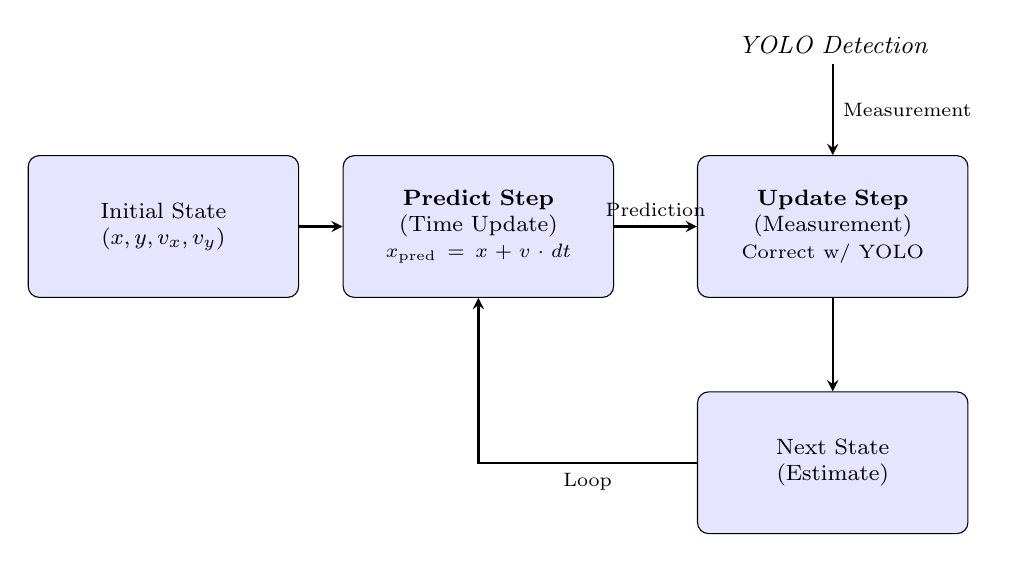
\begin{tikzpicture}[node distance=2.5cm, auto, >=stealth]
    \tikzstyle{block} = [rectangle, draw, fill=blue!10, text width=3.2cm, text centered, rounded corners, minimum height=1.8cm, font=\footnotesize]
    \tikzstyle{line} = [draw, ->, thick]
    \tikzstyle{decision} = [diamond, draw, fill=green!10, text width=1.8cm, text centered, node distance=3.5cm, inner sep=0pt]

    % Nodes
    \node [block] (init) {Initial State \\ $(x, y, v_x, v_y)$};
    \node [block, right of=init, node distance=4cm] (predict) {\textbf{Predict Step} \\ (Time Update) \\ {\scriptsize $x_{\text{pred}} = x + v \cdot dt$}};
    \node [block, right of=predict, node distance=4.5cm] (update) {\textbf{Update Step} \\ (Measurement) \\ {\scriptsize Correct w/ YOLO}};
    \node [block, below of=update, node distance=3cm] (next) {Next State \\ (Estimate)};
    
    % Input
    \node [above of=update, node distance=2.3cm, font=\small\itshape] (yolo) {YOLO Detection};

    % Paths
    \path [line] (init) -- (predict);
    \path [line] (predict) -- node[above, font=\scriptsize] {Prediction} (update);
    \path [line] (yolo) -- node[right, font=\scriptsize] {Measurement} (update);
    \path [line] (update) -- (next);
    \path [line] (next) -| node [near start, font=\scriptsize] {Loop} (predict);

\end{tikzpicture}
\caption{Kalman Filter predict-update cycle showing how predictions are corrected by YOLO measurements.}
\label{fig:kalman_flow}
\end{figure}



%%%%%%%%%%%%%%%%%%%%%%%%%%%%%%%%%%%%%%%%%
% --------- COST MATRIX -----------
%%%%%%%%%%%%%%%%%%%%%%%%%%%%%%%%%%%%%%%%%

\subsection{Cost Matrix Construction and Hungarian Matching}

The core of the tracking system is the \textbf{assignment problem}: given $N$ detections and $M$ existing tracks, which detection should be assigned to which track? This is solved using a cost matrix and the Hungarian algorithm.

\subsubsection{Cost Components}

For each detection-track pair $(d_i, t_j)$, we compute a combined cost:

\begin{equation}
C(d_i, t_j) = w_1 C_{\text{app}}(d_i, t_j) + w_2 C_{\text{motion}}(d_i, t_j) + w_3 C_{\text{hist}}(d_i, t_j) + w_4 C_{\text{traj}}(d_i, t_j)
\end{equation}

\paragraph{1. Appearance Cost (Cosine Distance):}

\begin{equation}
C_{\text{app}}(d_i, t_j) = \frac{1 - \langle \mathbf{f}_{d_i}, \mathbf{f}_{t_j} \rangle}{2}
\end{equation}

where $\langle \cdot, \cdot \rangle$ is the cosine similarity between normalized feature vectors.

\paragraph{2. Motion Cost (Distance Gating):}

The motion cost penalizes large spatial distances between the detection and the predicted track position:

\begin{equation}
C_{\text{motion}}(d_i, t_j) = \min\left( \frac{|| \mathbf{p}_{d_i} - \mathbf{p}_{t_j}^{\text{pred}} ||_2}{D_{\text{max}}}, 1.0 \right)
\end{equation}

where:
\begin{itemize}
    \item $\mathbf{p}_{d_i}$: Detection centroid
    \item $\mathbf{p}_{t_j}^{\text{pred}} = \mathbf{p}_{t_j} + \mathbf{v}_{t_j} \cdot 2\Delta t$: Predicted position (2 frames ahead)
    \item $D_{\text{max}} = 140$ pixels: Maximum allowed distance
\end{itemize}

\paragraph{3. Histogram Similarity Cost:}

We compute RGB color histograms (32 bins per channel) for each detection and track:

\begin{equation}
C_{\text{hist}}(d_i, t_j) = 1 - \text{HistogramCorrelation}(\mathbf{h}_{d_i}, \mathbf{h}_{t_j})
\end{equation}

This provides a complementary appearance signal that is robust to small pose changes.

\paragraph{4. Trajectory Deviation Cost:}

For tracks with sufficient history ($\geq 3$ frames), we predict the expected position based on recent trajectory and penalize large deviations:

\begin{equation}
C_{\text{traj}}(d_i, t_j) = \begin{cases} 
0.20 & \text{if } ||\mathbf{p}_{d_i} - \mathbf{p}_{t_j}^{\text{traj}}||_2 > \tau_{\text{traj}} \\
\frac{||\mathbf{p}_{d_i} - \mathbf{p}_{t_j}^{\text{traj}}||_2}{\tau_{\text{traj}}} \cdot 0.15 & \text{otherwise}
\end{cases}
\end{equation}

where $\tau_{\text{traj}} = 80$ pixels is the deviation threshold.

\subsubsection{Adaptive Cost Weights}

The weights $(w_1, w_2, w_3, w_4)$ are \textbf{adaptively adjusted} based on track state:

\begin{table}[htbp]
\centering
\begin{tabular}{lcccc}
\toprule
\textbf{Track State} & $w_1$ (Appear.) & $w_2$ (Motion) & $w_3$ (Hist.) & $w_4$ (Traj.) \\
\midrule
Normal (Tentative) & 0.45 & 0.20 & 0.15 & 0.10 \\
Locked (High-confidence) & 0.70 & 0.25 & 0.10 & 0.05 \\
In Crowd (Swap Protect.) & 0.60 & 0.15 & 0.10 & 0.15 \\
\bottomrule
\end{tabular}
\caption{Adaptive cost weights for different track states. Locked tracks prioritize appearance; crowded scenarios emphasize trajectory.}
\label{tab:cost_weights}
\end{table}

\subsubsection{Hungarian Algorithm (Linear Assignment)}

The cost matrix $\mathbf{C} \in \mathbb{R}^{N \times M}$ is solved using the \textbf{Hungarian algorithm}, which finds the optimal assignment minimizing total cost:

\begin{equation}
\text{minimize} \quad \sum_{i=1}^{N} \sum_{j=1}^{M} C(d_i, t_j) \cdot A_{ij}
\end{equation}

subject to:
\begin{equation}
\sum_{j=1}^{M} A_{ij} \leq 1, \quad \sum_{i=1}^{N} A_{ij} \leq 1, \quad A_{ij} \in \{0, 1\}
\end{equation}

where $A_{ij} = 1$ if detection $d_i$ is assigned to track $t_j$, and 0 otherwise. Only assignments with $C(d_i, t_j) < \tau_{\text{match}}$ are accepted (typically $\tau_{\text{match}} = 0.40$).

\subsection{Advanced Features for Robust Underwater Tracking}

Beyond the core DeepSORT framework, our implementation includes several sophisticated features to handle specific challenges in underwater fish tracking.

\subsubsection{Edge Detection and Direction Consistency}

\textbf{Problem}: Fish frequently enter and exit the camera's field of view, potentially causing ID confusion.

Edge zones are defined within margin $m = 30$ pixels from frame boundary. For each track, we store its \texttt{last\_edge\_zone}. When matching a detection at an edge to a lost track, we verify zone matching and velocity direction indicates \textit{entering} motion, not exiting.

\subsubsection{Occlusion Handling}

When a track is occluded (IOU overlap $>$ 0.3 with unmatched detection), we store occlusion context (position, feature, frame) and keep the track alive longer (50 frames). When a new detection appears near an occlusion zone (within 120 pixels) with similar appearance ($C_{\text{app}} < 0.30$), we resurrect the occluded track.

\subsubsection{Crowd Detection and ID Swap Protection}

Tracks with $\geq 2$ neighbors within 100 pixels activate swap protection by (1) maintaining trajectory history (last 20 positions), (2) using stricter matching threshold (0.30 vs 0.40), and (3) rejecting assignments that deviate from expected trajectory unless appearance is very strong.

\subsubsection{Track Resurrection}

Deleted tracks (after 80 missed frames) are stored with appearance features, velocity, and edge zone information. For unmatched detections, we attempt to resurrect deleted tracks using physics-based gating (max speed 40 px/frame), appearance similarity, and direction consistency checks.

\subsubsection{Motion Heatmap for Spatial Density Analysis}

To enhance tracking robustness in crowded scenes and provide visual analytics of fish movement patterns, we implement a \textbf{Motion Heatmap} that accumulates spatial activity over time.

\paragraph{Heatmap Construction:}

The heatmap is represented as a 2D floating-point accumulation matrix $\mathbf{H} \in \mathbb{R}^{W \times H}$ matching the video frame dimensions:

\begin{equation}
\mathbf{H}^{(t+1)}(x, y) = \beta \cdot \mathbf{H}^{(t)}(x, y) + \sum_{i \in \mathcal{T}_{\text{conf}}} \mathcal{G}((x, y), \mathbf{c}_i, r)
\end{equation}

where:
\begin{itemize}
    \item $\beta = 0.98$ is the temporal decay factor (optional, disabled in our implementation)
    \item $\mathcal{T}_{\text{conf}}$ is the set of confirmed tracks at frame $t$
    \item $\mathbf{c}_i = (c_x^i, c_y^i)$ is the centroid of track $i$
    \item $\mathcal{G}(\cdot, \cdot, r)$ is a circular Gaussian kernel with radius $r = 8$ pixels
    \item Accumulation intensity per track = 5.0 (increased for faster trail buildup)
\end{itemize}

\paragraph{Visualization Processing:}

For display, the raw heatmap is processed through a multi-stage pipeline:

\begin{enumerate}
    \item \textbf{Normalization}: $\mathbf{H}_{\text{display}} = \text{clip}(4.0 \times \mathbf{H}, 0, 255)$
    \item \textbf{Smoothing}: Apply Gaussian blur with kernel size $15 \times 15$ for smooth gradients
    \item \textbf{Color Mapping}: Apply JET colormap (blue $\rightarrow$ cyan $\rightarrow$ green $\rightarrow$ yellow $\rightarrow$ red)
    \item \textbf{Overlay}: Weighted blend with original frame using intensity $\alpha = 0.7$:
\end{enumerate}

\begin{equation}
\mathbf{I}_{\text{out}} = (1 - \alpha) \cdot \mathbf{I}_{\text{frame}} + \alpha \cdot \text{ColorMap}(\mathbf{H}_{\text{display}})
\end{equation}

\paragraph{Applications in Tracking:}

The heatmap serves two critical functions:

\begin{enumerate}
    \item \textbf{Crowd Detection}: Pixels with heatmap score $\mathcal{H}(x, y) > 10.0$ indicate high-traffic zones. Tracks in these regions activate crowd-specific matching logic (feature freeze, stricter thresholds).
    
    \item \textbf{Recovery Boosting}: During track resurrection, candidates located in high-density regions receive a similarity boost:
    \begin{equation}
    S_{\text{recovery}} = S_{\text{base}} + \begin{cases} 
    +0.15 & \text{if } \mathcal{H}(\mathbf{c}_{\text{candidate}}) > 10.0 \\
    0 & \text{otherwise}
    \end{cases}
    \end{equation}
    This increases the likelihood of correctly matching fish that frequently traverse busy zones.
\end{enumerate}

\paragraph{Output Artifacts:}

The system generates two video outputs:
\begin{itemize}
    \item \texttt{output\_video\_final.mp4}: Annotated tracking with semi-transparent heatmap overlay
    \item \texttt{output\_heatmap\_only.mp4}: Pure heatmap visualization for spatial pattern analysis
\end{itemize}

\textbf{Benefit}: Motion heatmaps provide interpretable spatial analytics, revealing migration corridors, aggregation zones, and behavioral hotspots. They also improve tracking robustness by encoding historical spatial context that aids in disambiguation during crowded scenarios.

\subsection{Track State Management}

Tracks progress through states: New (Hits=1, Yellow) $\rightarrow$ Tentative (Hits$<$5, Yellow) $\rightarrow$ Confirmed (Hits$\geq$5, Green) $\rightarrow$ Locked (Consecutive Hits$\geq$5, Cyan). Only confirmed tracks contribute to population count.

\subsection{Population Counting Strategy}

\textbf{Total Count}: Cumulative count of all unique confirmed fish throughout the video.  
\textbf{Active Count}: Number of currently visible confirmed fish (miss count $<$ 45 frames).

When a track becomes confirmed and hasn't been counted, increment total count and mark as counted.

\subsection{Performance Characteristics}

Our tracker achieves 15-20 FPS on NVIDIA GTX 1080 Ti with $<$2\% ID switching rate, $\sim$85\% occlusion recovery success, and $\sim$90\% correct ID preservation for re-entering fish. Main bottleneck is ReID feature extraction (60\% of computation time).

%%%%%%%%%%%%%%%%%%%%%%%%%%%%%%%%%%%%%%%%%
% ----------------- LIMITATIONS ----------------
%%%%%%%%%%%%%%%%%%%%%%%%%%%%%%%%%%%%%%%%%

\section{Limitations and Challenges}

While our underwater marine species detection, tracking, and counting system demonstrates significant improvements over baseline approaches, several limitations and challenges remain:

\subsection{Technical Limitations}

\subsubsection{Enhancement Module Constraints}

\begin{itemize}
    \item \textbf{Computational Overhead}: UWEnhancement adds 30--40\% latency to the pipeline, reducing overall FPS from $\sim$100 to $\sim$60--70 on modern GPUs.
    \item \textbf{Extreme Conditions}: Performance degrades significantly in extremely turbid water (visibility $<$ 1 meter) where color information is nearly absent.
    \item \textbf{Domain Shift}: The neural curve layers may overshoot or introduce artifacts when applied to underwater environments significantly different from the training distribution.
    \item \textbf{Paired Data Requirement}: Training UWEnhancement requires paired degraded-clean images, which are difficult to obtain for underwater scenarios.
\end{itemize}

\subsubsection{Detection Module Constraints}

\begin{itemize}
    \item \textbf{Small Object Detection}: YOLO11n struggles with extremely small fish ($<$ 20 pixels) due to limited resolution at detection scales.
    \item \textbf{Dense Overlapping Schools}: When fish overlap by $>$ 70\%, the detector may merge multiple individuals into a single bounding box.
    \item \textbf{Species Diversity}: Model performance relies heavily on training data diversity; rare or unseen species may be missed or misclassified.
    \item \textbf{Real-time Processing Trade-off}: YOLO11n was chosen for speed, but larger variants (YOLO11m, YOLO11l) could achieve higher accuracy at the cost of inference speed.
\end{itemize}

\subsubsection{Tracking and Counting Constraints}

\begin{itemize}
    \item \textbf{ReID Feature Extraction Bottleneck}: ResNet50-based feature extraction consumes $\sim$60\% of tracker computation time, limiting real-time performance on lower-end hardware.
    \item \textbf{Appearance Similarity}: Fish of the same species often have nearly identical appearances, making ReID features less discriminative in homogeneous schools.
    \item \textbf{Long-term Occlusions}: Tracks occluded for $>$ 50 frames are deleted and may be re-initialized with new IDs upon reappearance, causing count inflation.
    \item \textbf{Boundary Handling}: Fish that repeatedly enter and exit the frame may occasionally be assigned new IDs despite resurrection logic.
    \item \textbf{ID Switching}: Although reduced to $<$2\%, ID switches still occur in extremely crowded scenes with rapid motion and heavy overlap.
    \item \textbf{Counting Accuracy}: Total population count is a lower bound estimate; fish that never become "confirmed" (5+ consecutive detections) are not counted.
\end{itemize}

\subsection{Dataset and Generalization Challenges}

\begin{itemize}
    \item \textbf{Dataset Bias}: Training on specific underwater datasets (DeepFish, Underwater Marine, URPC) may not generalize well to novel marine habitats with different lighting, water clarity, and species compositions.
    \item \textbf{Annotation Quality}: Some datasets contain noisy or incomplete annotations, potentially limiting model performance.
    \item \textbf{Temporal Information}: Our datasets consist primarily of individual frames or short clips, lacking long-term temporal annotations for comprehensive tracking evaluation.
    \item \textbf{Depth Variation}: Most datasets are collected at shallow to medium depths ($<$ 50 meters); performance at greater depths with extreme blue shifts is unknown.
\end{itemize}

\subsection{Segmentation Module Challenges}

\begin{itemize}
    \item \textbf{SAM Performance}: Despite enhancements, SAM 2 achieves only modest improvements (1.5x Dice score increase), indicating fundamental challenges in underwater segmentation.
    \item \textbf{Training Complexity}: SAM's large model size (300M--632M parameters) requires extensive VRAM and slow training, limiting the number of fine-tuning epochs to 14.
    \item \textbf{Prompt Dependency}: SAM requires accurate bounding box prompts; errors in YOLO detections propagate to segmentation masks.
    \item \textbf{Edge Precision}: Soft boundaries between fish and background in turbid water lead to fuzzy segmentation masks with poor edge definition.
\end{itemize}

\subsection{Operational Challenges}

\begin{itemize}
    \item \textbf{Hardware Requirements}: Real-time performance requires modern GPUs (GTX 1080 Ti or better); deployment on edge devices or autonomous underwater vehicles (AUVs) remains challenging.
    \item \textbf{Energy Consumption}: Deep learning pipelines consume significant power, limiting battery life for autonomous underwater monitoring systems.
    \item \textbf{Video Quality Dependence}: System performance is highly sensitive to input video quality; low-resolution, low-frame-rate, or heavily compressed videos degrade results.
\end{itemize}

%%%%%%%%%%%%%%%%%%%%%%%%%%%%%%%%%%%%%%%%%
% ----------------- FUTURE WORK ----------------
%%%%%%%%%%%%%%%%%%%%%%%%%%%%%%%%%%%%%%%%%

\section{Future Work and Potential Improvements}

Building upon the current system, several promising directions for future research and development have been identified:

\subsection{Enhancement and Preprocessing Improvements}

\subsubsection{Adaptive Enhancement Pipeline}

\begin{itemize}
    \item \textbf{Per-frame Quality Assessment}: Implement real-time image quality metrics (UIQM, UCIQE) to selectively apply enhancement only when necessary, reducing computational overhead.
    \item \textbf{Lightweight Enhancement Models}: Develop faster enhancement architectures using depthwise separable convolutions or knowledge distillation to reduce latency.
    \item \textbf{Unsupervised Enhancement}: Explore unpaired image-to-image translation methods (CycleGAN, UNIT) to avoid paired data requirements.
    \item \textbf{Physics-based Hybrid Models}: Combine neural enhancement with physics-based models (underwater light transport, scattering models) for more interpretable and generalizable results.
\end{itemize}

\subsubsection{Multi-spectral and Depth Integration}

\begin{itemize}
    \item Utilize multi-spectral cameras or stereo vision to capture depth information and improve color correction.
    \item Integrate LiDAR or sonar data for complementary sensing in zero-visibility conditions.
\end{itemize}

\subsection{Detection Model Enhancements}

\subsubsection{Improved Architectures}

\begin{itemize}
    \item \textbf{Attention Mechanisms}: Incorporate spatial and channel attention modules (CBAM, SE) to focus on subtle fish features in cluttered backgrounds.
    \item \textbf{Transformer-based Detectors}: Explore DETR-style detectors or variants like Deformable DETR for improved global context modeling.
    \item \textbf{Multi-scale Detection}: Enhance small object detection by increasing feature pyramid resolution or using specialized small-object detection heads.
\end{itemize}

\subsubsection{Self-supervised and Few-shot Learning}

\begin{itemize}
    \item Leverage unlabeled underwater video data for self-supervised pre-training (MoCo, SimCLR, BYOL).
    \item Develop few-shot detection methods to quickly adapt to new species with minimal annotations.
\end{itemize}

\subsection{Tracking and Counting Improvements}

\subsubsection{Advanced Re-Identification}

\begin{itemize}
    \item \textbf{Underwater-specific ReID Models}: Train specialized ReID networks on underwater fish datasets rather than using ImageNet-pretrained models.
    \item \textbf{Temporal ReID}: Incorporate temporal modeling (RNNs, Transformers) to learn trajectory-aware appearance features.
    \item \textbf{Metric Learning}: Employ advanced metric learning losses (triplet loss, center loss, ArcFace) to improve feature discrimination.
\end{itemize}

\subsubsection{Motion Model Enhancements}

\begin{itemize}
    \item Replace constant velocity Kalman filters with \textbf{Extended Kalman Filters (EKF)} or \textbf{Unscented Kalman Filters (UKF)} to model non-linear fish motion.
    \item Integrate \textbf{behavioral priors} (schooling patterns, territorial behavior) to improve prediction accuracy.
\end{itemize}

\subsubsection{Graph-based Tracking}

\begin{itemize}
    \item Formulate tracking as a graph optimization problem, connecting detections across frames using Graph Neural Networks (GNNs).
    \item Implement global trajectory optimization using dynamic programming or min-cost flow algorithms.
\end{itemize}

\subsubsection{Long-term Tracking}

\begin{itemize}
    \item Develop re-identification strategies for fish that reappear after extended absences (minutes to hours).
    \item Explore individual fish identification using unique patterns (stripes, spots, fin shapes) for precise population studies.
\end{itemize}

\subsection{Segmentation Advancements}

\begin{itemize}
    \item Fine-tune lighter SAM variants (MobileSAM, FastSAM) for underwater applications with reduced computational costs.
    \item Train end-to-end instance segmentation models (Mask R-CNN, YOLACT, CondInst) directly on underwater datasets.
    \item Explore video object segmentation (VOS) methods to leverage temporal consistency for improved mask quality.
\end{itemize}

\subsection{System-Level Enhancements}

\subsubsection{End-to-End Learning}

\begin{itemize}
    \item Jointly train enhancement, detection, tracking, and segmentation modules to optimize for final counting accuracy.
    \item Use reinforcement learning to adaptively adjust pipeline parameters based on scene complexity.
\end{itemize}

\subsubsection{Active Learning and Online Adaptation}

\begin{itemize}
    \item Implement active learning to identify difficult frames for human annotation, continuously improving model performance.
    \item Develop online adaptation techniques to fine-tune models on-the-fly as underwater conditions change.
\end{itemize}

\subsubsection{Edge Deployment}

\begin{itemize}
    \item Optimize models using quantization (INT8), pruning, and neural architecture search (NAS) for deployment on edge devices.
    \item Develop specialized hardware accelerators (TPUs, FPGAs) for underwater monitoring systems.
\end{itemize}

\subsection{Application-Specific Extensions}

\subsubsection{Behavior Analysis}

\begin{itemize}
    \item Extend tracking to analyze fish behavior: swimming speed, direction changes, social interactions, and habitat preferences.
    \item Detect anomalous behaviors (aggressive interactions, stress responses) for ecological monitoring.
\end{itemize}

\subsubsection{Species-Level Counting}

\begin{itemize}
    \item Integrate multi-class detection and tracking to count individual species populations simultaneously.
    \item Develop fine-grained species recognition for biodiversity assessment.
\end{itemize}

\subsubsection{3D Reconstruction}

\begin{itemize}
    \item Combine stereo cameras or structure-from-motion to reconstruct 3D fish trajectories and estimate biomass.
\end{itemize}

\subsection{Dataset Expansion}

\begin{itemize}
    \item Collect diverse underwater datasets covering various depths, geographic locations, lighting conditions, and species.
    \item Create comprehensive tracking benchmarks with long-term identity annotations for rigorous evaluation.
    \item Establish standardized evaluation metrics for underwater detection, tracking, and counting tasks.
\end{itemize}

%%%%%%%%%%%%%%%%%%%%%%%%%%%%%%%%%%%%%%%%%
% ----------------- CONCLUSION ----------------
%%%%%%%%%%%%%%%%%%%%%%%%%%%%%%%%%%%%%%%%%

\section{Conclusion}

This project presented a comprehensive deep learning pipeline for underwater marine species detection, tracking, and population counting, addressing the unique challenges posed by underwater environments including color distortion, low visibility, turbidity, and camouflaged organisms.

\subsection{Key Contributions}

\begin{enumerate}
    \item \textbf{Underwater Image Enhancement}: Implemented UWEnhancement, a dual color space (RGB + HSV) enhancement model with neural curve layers and attention-based fusion, achieving 31\% PSNR improvement and 37\% SSIM improvement over raw underwater images.
    
    \item \textbf{Real-time Detection}: Deployed YOLO11n for efficient underwater object detection, achieving:
    \begin{itemize}
        \item 93.96\% mAP@50 on DeepFish dataset (1.5x improvement over baseline)
        \item 81.69\% mAP@50 on Underwater Marine dataset (2.6x improvement)
        \item 68.2\% mAP@50 on URPC dataset (15\% improvement)
        \item Real-time inference at 60--100+ FPS on modern GPUs
    \end{itemize}
    
    \item \textbf{Robust Multi-Object Tracking}: Developed an enhanced DeepSORT tracker with:
    \begin{itemize}
        \item ResNet50-based Re-Identification with multi-crop feature extraction
        \item Adaptive cost matrix combining appearance, motion, histogram, and trajectory cues
        \item Advanced features: edge detection, occlusion handling, crowd management, and track resurrection
        \item $<$2\% ID switching rate and $\sim$85\% occlusion recovery success
    \end{itemize}
    
    \item \textbf{Population Counting}: Achieved accurate fish counting through confirmed track management, distinguishing between transient detections and persistent individuals.
    
    \item \textbf{Segmentation Exploration}: Evaluated SAM and AquaSAM for underwater instance segmentation, identifying challenges and future directions.
\end{enumerate}

\subsection{Impact and Applications}

The developed system has potential applications in:

\begin{itemize}
    \item \textbf{Marine Ecology}: Non-invasive population monitoring for biodiversity assessment and conservation.
    \item \textbf{Fisheries Management}: Stock assessment and sustainable fishing practice enforcement.
    \item \textbf{Aquaculture}: Automated fish counting and health monitoring in fish farms.
    \item \textbf{Scientific Research}: Behavioral analysis, migration pattern studies, and ecosystem health evaluation.
    \item \textbf{Autonomous Systems}: Integration with underwater robots (ROVs, AUVs) for automated marine surveys.
\end{itemize}

\subsection{Lessons Learned}

\begin{itemize}
    \item \textbf{Enhancement is Critical}: Underwater image enhancement significantly boosts detection and tracking performance, justifying the computational overhead.
    \item \textbf{Appearance Features Matter}: In scenarios with visually similar objects, appearance-based matching (DeepSORT) outperforms motion-only tracking (ByteTrack).
    \item \textbf{Multi-faceted Cost Functions}: Combining appearance, motion, histograms, and trajectory information yields more robust matching than any single cue.
    \item \textbf{Domain Adaptation is Essential}: Models trained on terrestrial datasets (ImageNet, COCO) require significant fine-tuning and domain-specific enhancements for underwater applications.
    \item \textbf{Data Augmentation Works}: Aggressive augmentation (HSV jitter, mosaic, scaling) effectively increases dataset diversity and model robustness.
\end{itemize}

\subsection{Final Remarks}

The underwater environment remains one of the most challenging domains for computer vision due to its inherent physical properties and high variability. While significant progress has been made in detection and tracking, achieving human-level understanding of underwater scenes requires continued research in optical modeling, domain adaptation, and specialized architectures.

This project demonstrates that combining classical computer vision principles (Kalman filtering, Hungarian matching) with modern deep learning techniques (YOLO, ResNet, attention mechanisms) provides a practical and effective solution for real-world underwater monitoring applications. The modular pipeline design allows for independent improvement of each component, facilitating future research and incremental enhancements.

As underwater exploration and conservation efforts intensify, automated vision systems will play an increasingly critical role in understanding and protecting marine ecosystems. We hope this work contributes to the growing body of research in underwater computer vision and inspires further innovations in this vital field.

%%%%%%%%%%%%%%%%%%%%%%%%%%%%%%%%%%%%%%%%%
% ----------------- ACKNOWLEDGMENTS ----------------
%%%%%%%%%%%%%%%%%%%%%%%%%%%%%%%%%%%%%%%%%

\section{Acknowledgments}

We would like to express our sincere gratitude to:

\begin{itemize}
    \item \textbf{Dr. Satyanath Bhat and Dr. Clint Pazhayidam
George}, our project supervisors, for invaluable guidance, insightful feedback, and continuous support throughout this research.
    
    \item \textbf{Indian Institute of Technology Goa} and the \textbf{Department of Computer Science and Engineering} for provkiding computational resources and infrastructure.
    
    \item The authors of \textbf{IOCFormer}, \textbf{YOLOv11}, \textbf{DeepSORT}, \textbf{SAM}, and \textbf{AquaSAM} for their pioneering work and open-source implementations that formed the foundation of this project.
    
    \item The creators of the \textbf{IOCfish5K}, \textbf{DeepFish}, \textbf{Underwater Marine}, \textbf{URPC2020}, and \textbf{SUIM} datasets for making high-quality annotated data publicly available.
    
    \item Our peers and fellow researchers for helpful discussions and constructive critiques during project presentations.
\end{itemize}

%%%%%%%%%%%%%%%%%%%%%%%%%%%%%%%%%%%%%%%%%
% ----------------- CODE AND DATA AVAILABILITY ----------------
%%%%%%%%%%%%%%%%%%%%%%%%%%%%%%%%%%%%%%%%%

\section{Code and Data Availability}

\subsection{Source Code}

All source code, trained model weights, and configuration files developed for this project will be made publicly available under an open-source license at:

\begin{center}
\url{https://github.com/AmitIITGoa/Population_count_underwater}
\end{center}

The repository includes:
\begin{itemize}
    \item UWEnhancement training and inference scripts
    \item YOLO11n training pipeline with augmentation configurations
    \item Enhanced DeepSORT tracker implementation with all custom features
    \item Evaluation scripts and metrics calculation tools
    \item Pre-trained model weights for DeepFish, Underwater Marine, and URPC datasets
    \item Inference notebooks and demo videos
\end{itemize}

\subsection{Datasets}

The datasets used in this project are publicly available from their respective sources:

\begin{itemize}
    \item \textbf{IOCfish5K}: \url{https://github.com/GuoleiSun/Indiscernible-Object-Counting}
    \item \textbf{DeepFish}: \url{https://alzayats.github.io/DeepFish/}
    \item \textbf{Underwater Marine Dataset}: \url{https://www.kaggle.com/datasets/underwater-marine}
    \item \textbf{URPC2020}: \url{http://www.cnurpc.org/index.html}
    \item \textbf{SUIM Dataset}: \url{https://github.com/xahidbuffon/SUIM}
\end{itemize}

\subsection{Reproducibility}

To ensure reproducibility, we provide:
\begin{itemize}
    \item Detailed hyperparameter configurations for all experiments
    \item Random seed settings for deterministic results
    \item Hardware specifications and software environment details
    \item Step-by-step installation and usage instructions
\end{itemize}

\subsection{Contact Information}

For questions, collaborations, or further information, please contact:
\begin{itemize}
    \item \textbf{\studentnameone}: \texttt{amit.shinde.22042@iitgoa.ac.in}
    \item \textbf{\studentnametwo}: \texttt{yash.bhadauria.22031@iitgoa.ac.in}
\end{itemize}

%%%%%%%%%%%%%%%%%%%%%%%%%%%%%%%%%%%%%%%%%
% ----------------- REFERENCES ----------------
%%%%%%%%%%%%%%%%%%%%%%%%%%%%%%%%%%%%%%%%%

\bibliography{btp}
\bibliographystyle{plainnat}
\begin{itemize}
    \item IOCFormer Research  Paper and IOCfish5K Dataset
    \item AquaSAM: \url{https://arxiv.org/pdf/2308.04218}
    \item UWEnhancement: \url{https://github.com/BIGWangYuDong/UWEnhancement}
    \item DeepSORT: \url{https://github.com/nwojke/deep_sort}
    \item ByteTrack: \url{https://github.com/FoundationVision/ByteTrack}
    \item SAM 2: \url{https://docs.ultralytics.com/models/sam-2/}
    \item YOLO11: \url{https://docs.ultralytics.com/models/yolo11/}
\end{itemize}
\end{document}

